% Created 2021-01-28 Thu 00:43
% Intended LaTeX compiler: pdflatex
\documentclass[11pt]{article}
\usepackage[utf8]{inputenc}
\usepackage[T1]{fontenc}
\usepackage{graphicx}
\usepackage{grffile}
\usepackage{longtable}
\usepackage{wrapfig}
\usepackage{rotating}
\usepackage[normalem]{ulem}
\usepackage{amsmath}
\usepackage{textcomp}
\usepackage{amssymb}
\usepackage{capt-of}
\usepackage{hyperref}
\usepackage{listings}
\usepackage{minted}
\author{Philipp Beer}
\date{\today}
\title{}
\hypersetup{
 pdfauthor={Philipp Beer},
 pdftitle={},
 pdfkeywords={},
 pdfsubject={},
 pdfcreator={Emacs 27.1 (Org mode 9.4)}, 
 pdflang={English}}
\begin{document}

\tableofcontents

\documentclass[12pt]{article}

\usepackage[top=2.5cm, left=2cm]{geometry}
\usepackage{graphicx}

\%\usepackage{fontspec}
\%\setmainfont{Times New Roman}

\usepackage{setspace}
\onehalfspacing

\usepackage{amsmath}
\usepackage{amsfonts}
\usepackage{amssymb}
\usepackage{amsthm}

\usepackage{bbold}
\usepackage[utf8]{inputenc}
\usepackage{luatex85}
\usepackage[english]{babel}

\usepackage{url}

\usepackage{graphics}
\graphicspath{ {./images/} }

\usepackage{listings}
\usepackage{xcolor}

\definecolor{codegreen}{rgb}{0,0.6,0}
\definecolor{codegray}{rgb}{0.5,0.5,0.5}
\definecolor{codepurple}{rgb}{0.58,0,0.82}
\definecolor{backcolour}{rgb}{0.95,0.95,0.92}

\lstdefinestyle{mystyle}{
    backgroundcolor=\color{backcolour},   
    commentstyle=\color{codegreen},
    keywordstyle=\color{magenta},
    numberstyle=\tiny\color{codegray},
    stringstyle=\color{codepurple},
    basicstyle=\ttfamily\footnotesize,
    breakatwhitespace=false,         
    breaklines=true,                 
    captionpos=b,                    
    keepspaces=true,                 
    numbers=left,                    
    numbersep=5pt,                  
    showspaces=false,                
    showstringspaces=false,
    showtabs=false,                  
    tabsize=2
}

\lstset{style=mystyle}


\newtheorem{definizione}{Definizione}
\newtheorem{proposizione}{Proposizione}
\newtheorem{lemma}{Lemma}
\newtheorem{teorema}{Teorema}


\DeclareMathOperator{\EX}\{\mathbb{E}\}
\DeclareMathOperator{\Id}\{\mathbb{1}\}
\DeclareMathOperator{\sign}{sign}
\DeclareMathOperator{\diag}{diag}
\DeclareMathOperator{\tr}{Tr}
\DeclareMathOperator*{\argmin}{arg\,min}
\DeclareMathOperator*{\argmax}{arg\,max}

\title{Flajolet Martin}
\begin{document}
%\titlepage
%\clearpage\null\newpage
%\tableofcontents
%\pagebreak
\clearpage\null\newpage
\section{Introduction}
The goal of this assignment is to implement the Flajolet-Martin algorithm to estimate the cardinalities of multisets of words for a variety of entries in the online encyclopedia Wikipedia. Specifically count the number of unique words in a wikipedia page.

\subsection{Motivation}
Counting unique elements is one of the fundamental activities in most computer applications. In their original paper \cite{bib:fm85} mentioned computational constraints as a reason to search for alternative ways of achieving a reasonably accurate estimate of cardinalities of multisets. Aside from this, today additional use cases have arisen, that make the utilization of the below introduced of \emph{Flajolet-Martin algorithm} interesting. As will shown the algorithm is capable of handling stream data while estimating the cardinalities of the transmitted dataset in a single pass.


\section{Resources}
\subsection{Programming Language}
For the implementation Python is chosen as programming language. Aside from its ubiquity it also offers a number of packages that can be utilized for the realization of this task. In particular the wikpedia package \cite{bib:goldsmith} can be used to read arbitrary wikipedia articles as it layed out in~\ref{subsec:data}. 

\subsection{Data set}
\label{subsec:data}
The resources for which unique items are to be counted are the unique words occcuring in \emph{Wikipedia} entries. Numerous options for processing accessing this data are available that fall into these main categories:
\begin{itemize}
  \item Scraping the website and processing the read html pages for their content
\item Downloading Wikipedia as a database as described in \cite{bib:wikidl}
  \item Utilizing a package that encapsulates the aforementioned activities and provides the data to the user
\end{itemize}

Downloading \emph{Wikipedia} as database is possible but requires large storage space (~11GB) and for the most part will not be used. The second option is also a larger challenge as it requires signficant preprocessing steps before the actual activities in the assignment can be carried out. Therefore the third option of a package that provides the page content as a data object appears to be the most straight forward approach. Additional pre-processing steps were applied to the page content. The data was:
\begin{itemize}
\item modified to lowercase only
\item exchange all non-word characters with whitespace character
\item exchange all digits with whitespace character
\item replace multi-whitespace characters with a single whitespace
\end{itemize}
To get an accurate word count the above steps appear to be sensible to avoid words that can be considered unique and may only be different because of that fact that they appear at the beginning of a sentence or not. Digits in this work are not considered words and hence replaced. Removing the whitespace characters ensures a clean dataset so that situations where elements are exchanged with whitespace are not counted multiple times.

In order to have access to arbitrary Wikipedia entries a readily available python package \emph{Wikipedia} is utilized and implemented as class that reads and digests wikipedia pages based on the search term provided by the class user.


\section{General Solution Approach}
\subsection{Data Ingestion}
In order to get be able to count the number of unique words in a \emph{Wikipedia} entry the \emph{WikiText} class is instanciated and provided a search term for which an entry is queried by the wikipedia-Python package and if found returns an object with the respective page content. In case a search term is provided that can not found or retrieved a \emph{PageError} is returned to the use.

Subsequently, the pre-processing activities are carried out and the data object is ready for analysis.

\subsection{Algorithm Execution}
After the data from the \emph{Wikipedia} page has been ingested and pre-processed a second class (\emph{FlajoletMartin}) is utilized on order to execute the counting of the number of the unique words within that article. The data stream is transferred from the wikipedia page content provided to the newly created object.

The implementation is of this class is described in~ref{sec:class}

\subsection{Verification}
In order to validate the veracity of the Flajolet-Martin algorithm implementation a second method for counting the unique number of words is implemented inside the \emph{WikiText} class. It is based on the "classical" approach of creating a Python set after the page content has been pre-processed and providing the length of the remaining set. Hence, this approach relies soly on Python "on-board" functionality and is used for the verification of the Flajolet-Martin implementation.


\section{Flajolet-Martin Algorithm}
\subsection{Introduction}
The \emph{Flajolet-Martin algorithm} builds on probabilities encountered in the use of hashing functions can provide reasonably accurate estimates of cardinalities in large datasets. It is built on the assumption that the records to be estimated can be hashed in a fitting pseudo-random manner.

\subsection{Basic Estimation Approach}
\label{subsec:basicappr}
The paper by Flajolet and Martin lays out the following required elements for the estimation process:
- A record denoted as
\begin{definition}
  x = (x_0, x_1, \dots, x_p)
\end{definition}
is hashed via
\begin{equation}\label{eq:hash}
  \emph{hash function}(x) = (M + N \sum\limits_{j = 0}^p ord(x_j) 128^j) mod 2^L
\end{equation}
which transforms words into integers (y) with a uniform distribution. These integers are considered in the bit form via:
\begin{equation}
  y = \sum_{k \ge 0} bit(y, k)2^k.
  \end{equation}
  
- The length of the bitmap vector is set as:
\begin{equation}
  L > log_2(n/nmap) + 4.
\end{equation}
The nmap value determines the number of bitmaps calculated for each word which are combined via a bitwise 'OR' statement to treat the standard deviation of R, which is leftmost zero position in the bitmap and usually has
\begin{definition}
  \sigma(R) \approx 1.12
\end{definition}
This dispersion results in an error roughly 1 binary order of magnitude.

\subsection{Results using the basic estimation approach}
With the implementation of the basic algorithm described in~\ref{subsec:basicappr} and the utilization of the correction method of averaging multiple bitmaps yielded fluctuating results.
The results still flucuated roughly one binary order of magnitude around the correct results also with use of nmap = 64

\subsection{Probabilistic Counting with Stochastic Averaging}
In their paper \cite{bib:fm85} Flajolet and Martin point an additional approach \emph{Probabilistics Counting with Stochastic Averaging} (PCSA) to improve the performance of the algorithmic result. In this modification the hashing function
\begin{definition}
  \alpha = h(x) mod m
\end{definition}
is utilized to determine in which bitmap is updated. The corresponding information is stored at
\begin{definition}
  h(x) div m \equiv \floor h(x)/m \floor
\end{definition}. In the final step the average between the different bitmaps is calculated using
\begin{equation}
  A = \frac{ R^{<1>} + R^{<2>} + \dots + R^{<m>}}m
\end{equation}.
Under the assumption that the distribution of the hashed words into the different lots is even, it can be expected that n/m elements fall into each lot so that
\begin{definition}
  \ (1/\varphi)2^A
\end{definition}
can be a reasonable approximation of n/m.

\section{Validation}
\subsection{Basic Setup}
\label{subsec:bassetup}
To validate the different aspects of the \emph{Flajolet-Martin} algorithm, 3 categories of \emph{Wikpedia} were defined:
\begin{center}
 \begin{tabular}{||c c c c||} 
 \hline
 Name & Range \\ [0.5ex] 
 \hline\hline
 Small & 0 - 1049 \\ 
 \hline
 Medium & 1050 - 2549 \\
 \hline
 Large & n > 2550 \\
 \hline
\end{tabular}
\end{center}
With this setup it is validated whether the performance of the basic \emph{Flajolet-Martin} approach compared to the \emph{PCSA} differs among different ranges of n.

\subsection{Wikipedia Entries}
The search queries chosen are a random list of \emph{Wikipedia} entries that fall into in~\ref{subsec:bassetup} mentioned categories. The list is as follows:
To validate the different aspects of the \emph{Flajolet-Martin} algorithm, 3 categories of \emph{Wikpedia} were defined:
\begin{center}
 \begin{tabular}{||c c c c||} 
 \hline
 Search Term & True Unique Values \\ [0.5ex] 
 \hline\hline
 List of fatal dog attacks in the United States (2010s) & 54  \\ 
 \hline
 Weisswurst & 265 \\
 \hline
 university of nicosia & 1035 \\
 \hline
data privacy & 1049 \\ 
 \hline
 Timeline of the Israeli–Palestinian conflict 2015 & 1406 \\
 \hline
covid & 1657 \\
 \hline
List of Crusades to Europe and the Holy Land & 2464 \\ 
 \hline
 michael jordan & 2529 \\
 \hline
 List of University of Pennsylvania people & 2928 \\
 \hline
Donald Trump & 4633 \\ 
 \hline
2020 Nagorno-Karabakh war & 4643 \\
 \hline
List of association football families & 5883 \\
 \hline   
 \end{tabular}
 \end{center}

\subsection{Results}
For each search term the two estimation algorithms were run 1.000 teams each to retrieve a sufficient sample to analyze the behavior of each estimation method.

\begin{figure}[t]
    \centering
    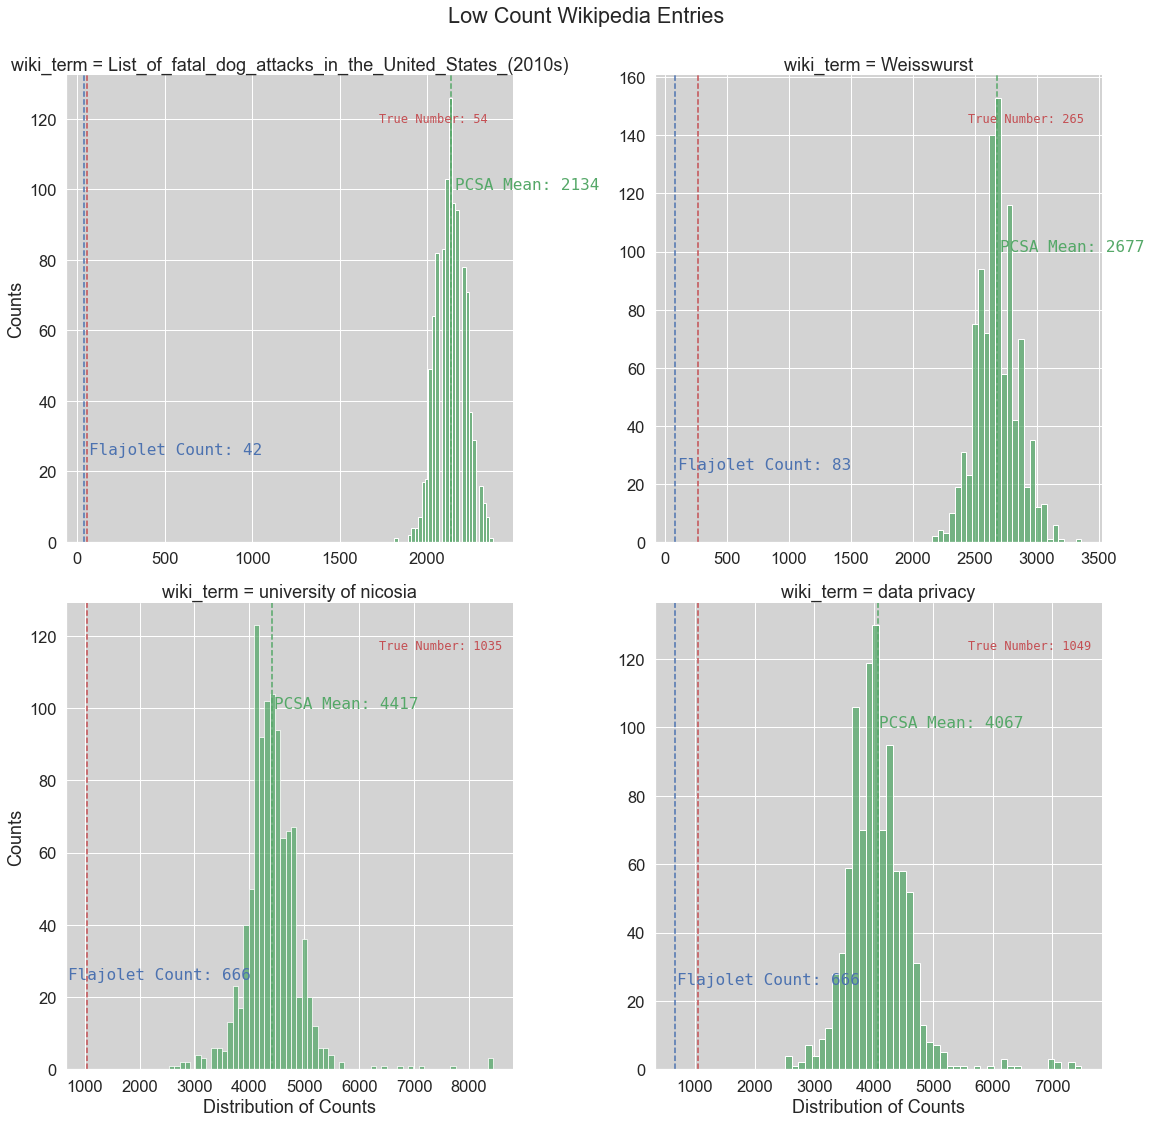
\includegraphics[width=0.99\textwidth]{distribution_small}
    \caption{Low Count - Distribution of Estimations}
    \label{fig:dist_small}
\end{figure}

\begin{figure}[t]
    \centering
    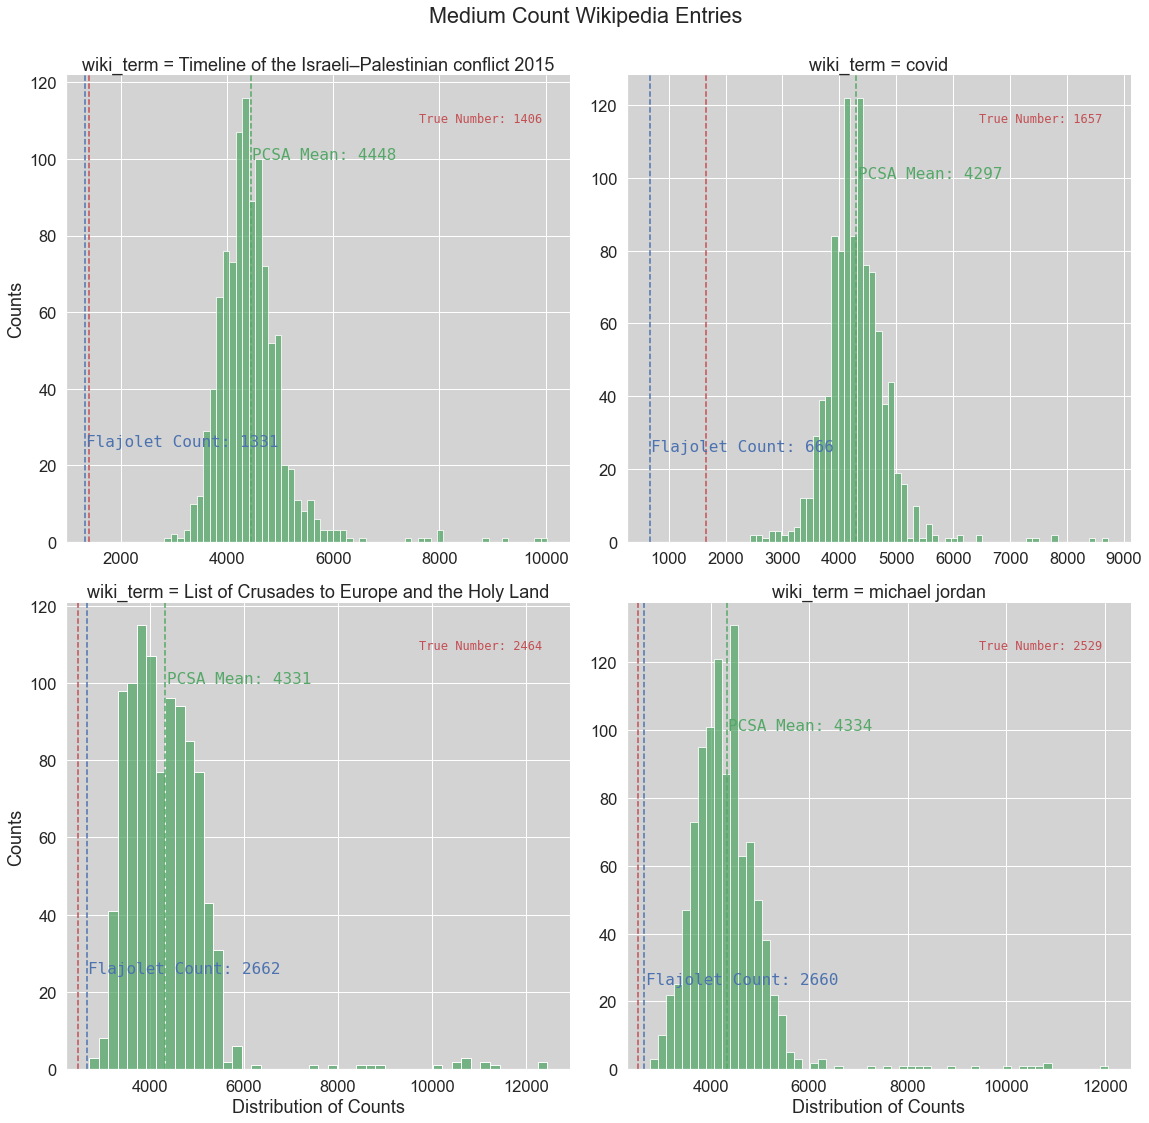
\includegraphics[width=0.99\textwidth]{distribution_med}
    \caption{Medium Count - Distribution of Estimations}
    \label{fig:dist_small}
\end{figure}

\begin{figure}[t]
    \centering
    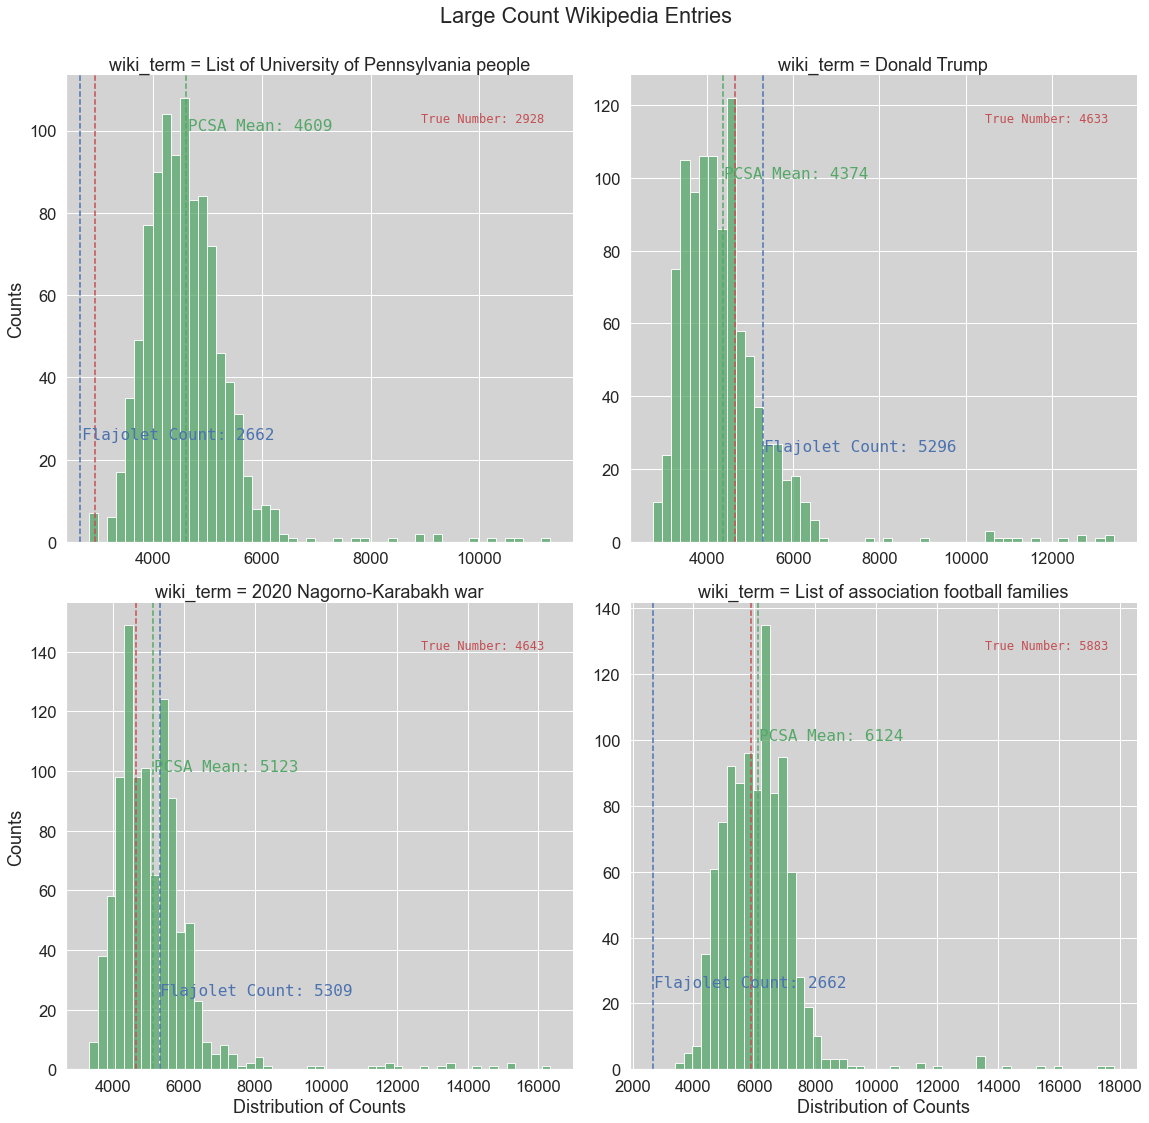
\includegraphics[width=0.99\textwidth]{distribution_large}
    \caption{High Count - Distribution of Estimations}
    \label{fig:dist_small}
\end{figure}



Several interesting observations can be made:
\begin{itemize}
\item The basic estimation method is much more stable in its behavior compared to the \emph{PCSA} implementation. The results are very consistent and in most cases do not deviate in their results over the 1.000 executions. The only variable factor during those executions are the chosen factors for the hash function \eref{eq:hash}.
\item The \emph{PCSA} has a large distribution and tends to overestimate results in some individual cases very significantly.
\item The \emph{PCSA} method performed worst within the low count category of the Wikipedia entries. In the worst case the algorithm was off by factor of 51.
\item As the number of unique entries increases the performance of the \emph{PCSA} method improves but still lags the basic estimation method. Only in the case of the of the query with the largest unique values in the sample set (List of assocation football families) the \emph{PCSA} outperforms the basic estimation method in terms of accuracy.
\item In the area of performance the \emph{PCSA} approach is significantly more performant compared to the basic estimation method.
\item Running the entire test scenario with 12 search terms, nmap = 64 and 1.000 executions per search term took roughly 180 minutes on a 4-core system with Hyper-Threading active and a very naive multi-threading implementation.
\end{itemize}

  
\subsection{Conclusion}
This implementation of the basic \emph{Flajolet-Martin} algorithm achieves mediocre results that are generally ok but in some instances (e.g. search terms covid, university of nicosia, data privacy) show to much deviation for most real-world applications. The \emph{PCSA} implementation performs significantly worse compared to the basic estimation. In general its performance improves as the number of unique items in the stream increases. In the range 4500 unique items is starts to enter the range predicted by Flajolet and Martin in ~/cite{fm85}.

The area of improvement appears to be proper choice of the hash function which does not produce reasonable results in its current state.


\section{Code}
\label{sec:class}

\subsection{Flajolet-Martin and Wikipedia Processing }
The implementation of both classes as well as the test run described above is as follows:
\begin{center}
\lstinputlisting[language=Python, caption=\emph{Flajolet-Martin} Implementation]{final_assignment.py}
\end{center}

\subsection{Visualization Code}
The visualization were done with slight variation of the following code:
\lstinputlisting[language=Python, caption=Visualization Code]{fm_analytics.py}

\pagebreak
\clearpage\null\newpage
\begin{thebibliography}{widest entry}
\bibitem[FM85]{bib:fm85} Flajolet M. and Martin G. N., ``Probabalistic Counting for Data Base Applications'', \emph{Journal of Compyter and System Sciences}, 1985
\bibitem[Py_Wiki]{bib:goldsmith} Goldsmith, J. ``Wikipedia'', \url{https://github.com/goldsmith/Wikipedia}
\bibitem[WikiDB] {bib:wikidl} Wikimedia Downloads \emph{https://dumps.wikimedia.org}, Wikimedia! The Wikimedia Foundation, Inc., 2021
\end{thebibliography}
\end{document}
